\section{Shell}

\begin{frame}[fragile]{Introduction to shell}
	\begin{itemize}
		\item A shell is a command-line interpreter that provides a user interface for accessing an operating system's services.
		\item It allows users to execute commands, manage files, and run programs through text-based inputs.
		\item Consider it as a direct communication channel between you and your computer's operating system.
	\end{itemize}
\end{frame}

\begin{frame}[fragile]{Types of shells}
	\begin{itemize}
		\item \textbf{Bash}: The Bourne Again Shell, the default shell on older macOS versions and most GNU/Linux systems.
		\item \textbf{Zsh}: An extended version of Bash with additional features like better auto-completion and theme support; the macOS default since Catalina.
	\end{itemize}
\end{frame}

\begin{frame}[fragile]{Why zsh?}
	\begin{itemize}
		\item Enhanced auto-completion for commands, file paths, and options
		\item Better customization options with themes and plugins
		\item Spelling correction and approximate completion
		\item macOS has made zsh the default shell since Catalina (10.15)
	\end{itemize}
\end{frame}

\begin{frame}[fragile]{macOS Terminal}
	\begin{itemize}
		\item \textbf{Terminal.app}: ships with macOS — find it in Applications $\rightarrow$ Utilities
		\item zsh is the default shell since Catalina (10.15), see ``Why zsh?'' above
		\item \textbf{iTerm2}: popular alternative with split panes, profiles and a hotkey window
		\item \textbf{oh-my-zsh}: plugin and theme manager for zsh, \href{https://ohmyz.sh}{ohmyz.sh}
	\end{itemize}
\end{frame}

\begin{frame}{File organization in macOS}
	\begin{center}
	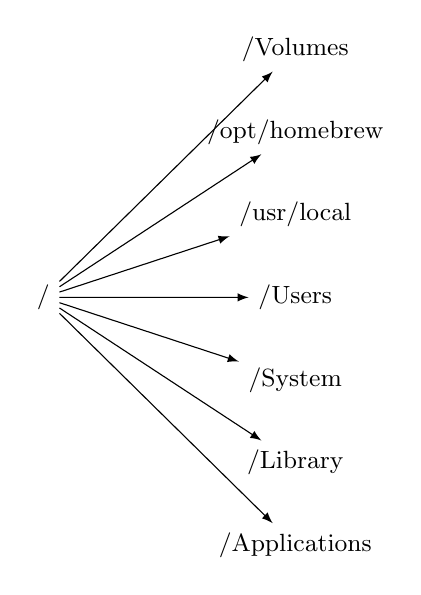
\begin{tikzpicture}[
		grow=right,
		level distance=3.2cm,
		level 1/.style={sibling distance=1.05cm},
		every node/.style={font=\small},
		edge from parent/.style={draw, -latex}
	]
	\node {/}
		child { node {/Applications} }
		child { node {/Library} }
		child { node {/System} }
		child { node {/Users} }
		child { node {/usr/local} }
		child { node {/opt/homebrew} }
		child { node {/Volumes} };
	\end{tikzpicture}
	\end{center}
\end{frame}

\begin{frame}[fragile]{File organization in macOS}
	\begin{itemize}
		\item \textbf{/Applications}: GUI apps, each an app bundle
		\item \textbf{/Library}: system-wide support files (fonts, frameworks)
		\item \textbf{/System}: macOS system files, protected by SIP
		\item \textbf{/Users/you}: your home — \textbf{~/Library} keeps per-user preferences and caches
		\item \textbf{/usr/local}: Homebrew prefix on Intel Macs
		\item \textbf{/opt/homebrew}: Homebrew prefix on Apple Silicon (see Package Manager)
		\item \textbf{/Volumes}: external disks and mounted .dmg images
	\end{itemize}

	For more detailed information, check \href{https://developer.apple.com/library/archive/documentation/FileManagement/Conceptual/FileSystemProgrammingGuide/FileSystemOverview/FileSystemOverview.html}{Apple's File System documentation}
\end{frame}

\begin{frame}[fragile]{Basic bash commands}
	\begin{itemize}
		\item \textbf{pwd}: Print working directory - shows your current location in the file system
		\item \textbf{ls}: List directory contents (files and folders)
		\item \textbf{cd}: Change directory - navigate between folders
		\item \textbf{mkdir}: Create a new directory
		\item \textbf{touch}: Create an empty file or update file timestamps
		\item \textbf{cp}: Copy files or directories
		\item \textbf{mv}: Move or rename files or directories
		\item \textbf{rm}: Remove files or directories
		\item \textbf{cat}: Concatenate files
		\item \textbf{echo}: Print text or variables to the terminal
		\item \textbf{>}: Redirect stdout to overwrite file
		\item \textbf{>>}: Redirect stdout to append file
	\end{itemize}
\end{frame}

\begin{frame}[fragile]{Practical examples}
	\begin{minted}{bash}
# Navigate to your home directory
cd ~

# List files in long format
ls -l

# Create a new directory
mkdir my_project

# Navigate into the directory
cd my_project

# Create a new file
touch README.md

# Copy a file
cp README.md README_copy.md

# Move/Rename a file
mv README_copy.md README_backup.md

# Remove a file
rm README_backup.md
	\end{minted}
\end{frame}

\begin{frame}[fragile]{Practical examples}
	\begin{minted}{bash}
cd ~/my_project
# redirect stdout into files
echo "fooo" >foo
echo "barrr" >bar

# concatenate two files
cat foo bar

# Go to parent path
cd ..

# Dangerous!!! You'd better use project like trash-cli
rm -rf my_project
	\end{minted}
\end{frame}
